\documentclass{report}
\usepackage[a4paper, right=2.5cm, left=2.5cm, top=2cm, bottom=2cm]{geometry}
\usepackage[utf8]{inputenc}
\usepackage{amsmath, amsfonts, amssymb, systeme}
\usepackage{stmaryrd}
\usepackage{graphicx}
\usepackage[numbers]{natbib}
\usepackage{hyperref}
\usepackage{float}
\usepackage{cleveref}

\usepackage{todonotes}

\hypersetup{
    colorlinks=true,
    linkcolor=blue,
    filecolor=magenta,      
    urlcolor=cyan,
    pdftitle={AS Projet ResNet},
    % pdfpagemode=FullScreen,
}
\urlstyle{same} %\href{url}{Text}

\newtheorem{theorem}{Théorème}
\newtheorem{proof}{Preuve}
\newtheorem{proposition}{Proposition}
\newtheorem{assumption}{Hypothèse}
\newtheorem{definition}{Définition}
\newtheorem{cor}{Corollaire}
\newtheorem{lem}{Lemme}
\newtheorem{note}{Note}
    
\title{Projet d'appentissage statistique\\Facteur de régulation des ResNets profonds}
\author{SHEN Pingya, VIN Charles}
\date{\today}

\begin{document}
\maketitle

\chapter{Introduction}
Avant l'introduction de ResNet en 2015 par He et al., l'architecture GoogLeNet était le dernier gagnant des challenges de vision par ordinateur. Cette architecture avait été développée pour pallier les problèmes d'apprentissage liés à l'augmentation de la profondeur de VGG, une autre architecture proéminente.

Un réseau plus profond peut offrir de meilleures performances dans certaines conditions, mais il est aussi sujet à des problèmes tels que l'explosion ou l'évanouissement du gradient de la loss. Durant la rétropropagation, les grandes ou petites valeurs de gradient peuvent s'amplifier à travers les couches du réseau, entraînant un gradient bien plus grand ou plus petit dans les dernières couches par rapport aux premières. Cet effet est multiplicatif et dépend donc de la profondeur du réseau.

Pour un réseau d'une profondeur $L$, on modélise ces états cachés de dimension $d$ par une séquence $(h_k)_{1 \leq k \leq L}$ avec $h_k \in \mathbb{R}^d, \forall 0 \leq k \leq L$. L'explosion du gradient peut être décrite mathématiquement par, avec une forte probabilité, $\left\| \frac{\partial \mathcal{L}}{\partial h_0} \right\| \gg \left\| \frac{\partial \mathcal{L}}{\partial h_L} \right\|$, où $\mathcal{L}$ représente la loss et $\left\| \cdot \right\|$ la norme euclidienne.

GoogLeNet, bien qu'offrant des une légère amélioration des performance par rapport à VGG, était encore relativement complexe et sa profondeur comparable à celle de VGG, passant de 22 à 16 couches. En 2015, ResNet a introduit un modèle allant jusqu'à 152 couches, divisant par deux le nombre d'erreurs de GoogLeNet. Son innovation réside dans l'intégration de \textit{skip connections} entre les couches successives, facilitant le passage du gradient au sein du réseau. Mathématiquement, cela donne la relation récurrente suivante pour la séquence $(h_k)_{1 \leq k \leq L}$ :
\[
    h_{k+1} = h_k + f(h_k, \theta_{k+1})
.\]

où $f(\cdot, \theta_{k+1})$ représente les transformations effectuées par la couche $k$ et paramétrées par $\theta_{k+1} \in \mathbb{R}^p$.

Les ResNets sont devenus la base de nombreux modèles d'apprentissage profond de pointe, s'étendant au-delà du traitement d'images pour inclure des domaines tels que le traitement du langage naturel et l'apprentissage par renforcement. L'idée des \textit{skip connections} a inspiré de nombreuses autres architectures et est devenue une pratique courante dans la conception des réseaux neuronaux profonds.

\begin{figure}[htbp]
    \centering
    % \includegraphics[width=.9\textwidth]{figs/}
    \caption{Illustration du modèle ResNet avec la présence de \textit{skip connections} dans chaque bloc.}
    \label{fig:resnet}
\end{figure}

Malgré ces avancées, ResNet rencontre toujours des problèmes de gradient durant l'apprentissage. La méthode traditionnelle pour contrer cela est la normalisation des états cachés après chaque couche (\textit{batch normalization}). Cependant, cette approche a un coût computationnel et dépend fortement de la taille du \textit{batch}. Une alternative est d'incorporer un facteur d'échelle $\alpha_L$ devant le terme résiduel, conduisant au modèle suivant :
\begin{equation}\label{resnet_equation}
    h_{k+1} = h_k + \alpha_L f(h_k, \theta_{k+1})
\end{equation}
Le choix de $\alpha_L$ est crucial et dépend naturellement de la profondeur $L$ du réseau. Il assure que la variance du signal reste stable lors de sa propagation à travers les couches. Cependant, il n'existe actuellement ni preuve formelle ni justification mathématique solide pour le choix de ce facteur de régularisation.

Dans ce cours, nous examinerons les fondements mathématiques pour choisir la valeur de $\alpha_L$ en fonction de $L$ et de la distribution initiale des poids, dans le but d'éviter les problèmes d'apprentissage. Deux axes principaux d'étude seront abordés :
\begin{enumerate}
    \item Le facteur $\alpha_L$ à l'initialisation : L'initialisation des paramètres est cruciale pour la phase d'apprentissage d'un modèle et influe même sur ses capacités de généralisation. Une mauvaise initialisation peut entraîner une divergence ou une disparition rapide du gradient, voire un blocage dans l'apprentissage. L'étude du rôle de $\alpha_L$ lors de l'initialisation est donc pertinente. Nous considérerons que, à l'initialisation, les poids de chaque couche $(\theta_k)_{1 \leq k \leq L}$ sont choisis de manière indépendante et identique selon une loi, typiquement gaussienne ou uniforme sur $\mathbb{R}^p$. 
    \item L'approche continue : Bien que le réseau neuronal soit constitué de nombreuses couches distinctes, l'ensemble du réseau peut être considéré comme une fonction, lorsqu'il y a suffisament de neurones. L'idée centrale des équations différentielles neuronales est de traiter les couches distincts du réseau comme continues, en supposant que chaque couche subit de petits changements. Ainsi, l'entrée de la couche suivante est considérée comme le résultat de l'intégrale de l'entrée de la couche précédente. Cela peut être comparé au mouvement d'un projet, où le déplacement dans la deuxième seconde peut être approximé par la déplacement dans la première seconde plus la vitesse dans la première seconde (multipliée par l'intervalle de temps d'une seconde).
    Les équations différentielles neuronales ont ouvert une nouvelle direction pour la théorie et la pratique de l’apprentissage profond et ont été appliquées à la classification d’images, aux séries chronologiques et à d’autres domaines. Tous les réseaux d'apprentissage profond avec des connexions résiduelles peuvent être exprimés approximativement par des équations différentielles neuronales
\end{enumerate}
\chapter*{Le facteur $\alpha_L$ à l'initialisation}

Dans cette section, notre objectif est d'examiner comment le facteur de mise à l'échelle $\alpha_L$ affecte la stabilité des ResNets lors de leur initialisation, en supposant que les poids sont des variables aléatoires indépendantes et identiquement distribuées (i.i.d.). Nous analyserons la modélisation, l'initialisation des paramètres et les hypothèses nécessaires à cette démarche.
% Faire un horizon de la partie "related works" en creusant plus loin ? 

\section{Modèle et hypothèses}
\subsection{Modèle}
Le modèle est basé sur un ensemble de données composé de $n$ paires $(x_i, y_i)_{1 \leq i \leq n}$ avec $x_i \in \mathbb{R}^{n_{\text{in}}}$ comme vecteur d'entrée et $y_i \in \mathbb{R}^{n_{\text{out}}}$ comme vecteur de sortie à prédire (soit en valeurs continues soit en format \textit{one-hot}). Soit $F_\pi(x) \in \mathbb{R}^{n_{\text{out}}}, x \in \mathbb{R}^{n_{\text{in}}}$ la sortie du ResNet définie par 
\begin{align*}
    h_0 &= Ax, \\
    h_{k+1} &= h_k + \alpha_L V_{k+1}g(h_k, \theta_k), \quad 0 \leq k \leq L - 1, \\
    F_{\pi}(x) &= Bh_L,
\end{align*}
où $\pi = (A, B, (\theta_k)_{k \leq L}, (V_k)_{1 \leq k \leq L})$ sont les paramètres du modèle avec $A \in \mathbb{R}^{d \times n_{\text{in}}}, B \in \mathbb{R}^{n_{\text{out}} \times d}, \theta_k \in \mathbb{R}^p$ et $V_k \in \mathbb{R}^{d \times d}$ pour $k = 1, \ldots, L$. La fonction $g : \mathbb{R}^d \times \mathbb{R}^p \to \mathbb{R}^d$ représente le choix de l'architecture d'un bloc du ResNet. Nous nous intéressons principalement à la suite des états cachés $(h_k)_{0 \leq k \leq L}$ et non aux changements de dimension permis par les matrices $A$ et $B$.
% Un aspect important du modèle \cite{torchvision2016} est que la fonction de couche prend la forme d'une multiplication matrice-vecteur, ce qui sera crucial pour utiliser les résultats de concentration sur des variables aléatoires ??????? Important ????????? 
Finalement, on définit $l: \mathbb{R}^{n_{\text{out}}} \times \mathbb{R}^{n_{\text{out}}} \to \mathbb{R}_+$ comme la fonction de \textit{loss}, différentiable par rapport à son premier paramètre. Cette \textit{loss} peut être une perte quadratique ou une entropie croisée. L'objectif de l'apprentissage est de trouver le paramètre optimal $\pi$ qui minimise le risque empirique $\mathcal{L}(\pi) = \sum_{i=1}^{n} l(F_\pi(x_i), y_i)$ à travers une descente de gradient stochastique ou l'une de ses variantes.

\subsection{Initialisation des paramètres} 
Nous rappelons que $\theta_k \in \mathbb{R}^p$ et $V_k \in \mathbb{R}^{d \times d}$ sont les paramètres des couches cachées de notre modèle pour tout $k \in \llbracket 1, L \rrbracket$. Ces paramètres sont choisis à l'initialisation comme la réalisation de variables aléatoires i.i.d., généralement suivant une distribution uniforme ou gaussienne. Cette initialisation est indépendante de $L$ et donc du modèle représenté par $g$, permettant de considérer plusieurs architectures différentes dans notre étude. Nous examinerons également d'autres approches dépendantes du modèle pour étudier le choix de $\alpha_L$ (par exemple, Yang et Schoenholz, 2017 ou Wang et al., 2022 \cite{torchvision2016}).

\subsection{Hypothèses}
Pour notre première hypothèse, nous avons besoin de la définition suivante :
\begin{definition}[Variable aléatoire $s^2$ sub-gaussienne]
    En théorie des probabilités, une distribution $s^2$ sub-gaussienne est une distribution de probabilité caractérisée par une décroissance rapide des queues de distribution. Bien qu'il existe de nombreuses définitions et propriétés, nous retiendrons dans ce cours la suivante : soit $X$ une variable aléatoire réelle,
    \[
        \forall \lambda \in \mathbb{R}, \mathbb{E}[\exp(\lambda X)] \leq \exp\left(\frac{\lambda^2 s^2}{2}\right).
    \]
    De manière informelle, les queues d'une distribution sub-gaussienne sont dominées par celles d'une distribution gaussienne, c'est-à-dire qu'elles décroissent au moins aussi rapidement.
\end{definition}

Avec cette définition en tête, passons aux hypothèses. Pour tout $ 1 \leq  k \leq L  $
\begin{assumption}\label{H1}
    Pour un certain $ s \geq 1 $, les entrées de  $ \sqrt{d}V_k $ sont des variables aléatoires symétriques i.i.d., $ s^2 $ sub-gaussiennes, indépendantes de $ d $ et $ L $ et de variance unitaire.
\end{assumption}
\begin{note}
    L'hypothèse \ref{H1} est en pratique satisfaite par toutes les initialisations, en particulier celle par défaut dans les paquets Keras \cite{torchvision2016} et Torch Vision \cite{torchvision2016}.
    % Cette hypothèse permet de .... dans la preuve ... ??
\end{note}

\begin{assumption}\label{H2}
    Pour un certain $ C > 0 $, indépendant de $ d $ et $ L $, et pour tout $ h \in \mathbb{R}^D  $ 
    \[
        \frac{\left\| h \right\| ^2}{2 } \leq  \mathbb{E }[ \left\|  g(h, \theta _ k ) \right\| ^2 ] \leq \left\| h \right\| ^2
    .\]
    and
    \[
        \mathbb{E } [\left\| g(h, \theta _k)  \right\| ^8 ]\leq C \left\| h  \right\| ^8
    .\]
\end{assumption}
\begin{note}
    La première partie de l'hypothèse \ref{H2} assure que $g(\cdot, \theta_{k+1})$ se comporte approximativement comme une isométrie en moyenne, c'est-à-dire qu'elle préserve les longueurs et les mesures d'angles entre son espace de départ et son espace d'arrivée.

    La deuxième partie de l'hypothèse \ref{H2} vise à limiter les variations excessives dans la norme de $g(h_k, \theta_{k+1})$.
\end{note}


% \begin{table}[h]
%     \centering
%     \begin{tabular}{lll}
%         \hline
%         \textbf{Nom} & \textbf{Récurrence} & \textbf{Paramètres} \\ \hline
%         res-1 & \( h_{k+1} = h_k + \alpha_L V_{k+1}\sigma(h_k) \) & \( \theta_{k+1} = \emptyset \) \\
%         res-2 & \( h_{k+1} = h_k + \alpha_L V_{k+1}\sigma(W_{k+1}h_k) \) & \( \theta_{k+1} = W_{k+1} \) \\
%         res-3 & \( h_{k+1} = h_k + \alpha_L V_{k+1}\text{ReLU}(W_{k+1}h_k) \) & \( \theta_{k+1} = W_{k+1} \) \\ \hline
%     \end{tabular}
%     \caption{Exemples d'architectures ResNet considérées dans l'article. Dans les deux premiers cas, la fonction d'activation \( \sigma \) est telle que, pour tout \( x \in \mathbb{R} \), \( a|x| \leq |\sigma(x)| \leq b|x| \), avec \( \frac{1}{\sqrt{2}} \leq a < b \leq 1 \). Dans les deux derniers cas, \( W_{k+1} \in \mathbb{R}^{d \times d} \).}
%     \label{tab:resnet_architectures}
% \end{table}

\section{Limite probabilistique de la norme des états cachés}

Dans cette section, nous nous intéressons à la quantité $ {\left\| h_L - h_0 \right\|} / {\left\| h_0 \right\|}$. Cette mesure permet d'analyser la valeur des états cachés entre le début et la fin du réseau. Si $\left\| h_L - h_0 \right\| \ll \left\| h_0 \right\|$, cela suggère que le réseau agit presque comme une fonction identité. À l'inverse, un ratio $\left\| h_L - h_0 \right\| \gg \left\| h_0 \right\|$ indique une explosion des valeurs des états cachés. Une situation équilibrée serait représentée par $\left\| h_L - h_0 \right\| \approx \left\| h_0 \right\|$.

Nous appliquerons un raisonnement similaire aux gradients avec la quantité ${\left\| \frac{\partial \mathcal{L}}{\partial h_0} - \frac{\partial \mathcal{L}}{\partial h_L} \right\|} / {\left\| \frac{\partial \mathcal{L}}{\partial h_L} \right\|}$. En raison de la propagation rétroactive du gradient qui commence à partir de la fin du réseau, cette mesure est comparée à la dernière valeur du gradient $\frac{\partial \mathcal{L}}{\partial h_L}$.

Les propositions et corollaires suivants décriront comment le rapport ${\left\| h_L - h_0 \right\|} / {\left\| h_0 \right\|}$ se comporte en fonction de $L\alpha_L$, en établissant différentes bornes supérieures et inférieures.


\begin{proposition}[Admise ? J'ai pas su la démontrer oof]\label{prop2}
    Considérons un ResNet \cite{torchvision2016} tel que les hypothèses \ref{H1} et \ref{H2} soient satisfaites.
    Si \( L\alpha_L^2 \leq 1 \), alors, pour tout \( \delta \in (0, 1) \), avec une probabilité d'au moins \( 1 - \delta \),
    \[
        \frac{\|h_L - h_0\|^2}{\|h_0\|^2} \leq \frac{2L\alpha_L^2}{\delta}
    .\]
\end{proposition}
La proposition \ref{prop2} par sa borne supérieur petite indique que le réseau se comporte comme une fonction identité dans le cas où $ L \alpha ^2 _L \ll 1 $.

\begin{proposition}[Admise]\label{prop3}
    Considérons un ResNet \cite{torchvision2016} tel que les hypothèses \ref{H1} et \ref{H2} soient satisfaites.
    \begin{itemize}
        \item[(i)] Supposons que $ d \geq 64 $ et $ \alpha _L ^2 \leq  \frac{2 }{(\sqrt{C } s^4 + 4 \sqrt{C } + 16 s ^4)d} $. Alors, pour tout $ \delta \in (0, 1) $, avec une probabilité d'au moins $ 1 - \delta $,
        \[
            \frac{\|h_L - h_0\|^2}{\|h_0\|^2} > \exp\left(\frac{3L\alpha_L^2}{8} - \sqrt{\frac{11L\alpha_L^2}{d\delta}}\right) - 1,
        \]
        à condition que
        \[
            2L \exp\left(-\frac{d}{64\alpha_L^2s^2}\right) \leq \frac{\delta}{11}.
        \]
        \item[(ii)] Supposons que $ \alpha_L^2 \leq \frac{1}{\sqrt{C}(d + 128s^4)} $. Alors, pour tout $ \delta \in (0, 1)$, avec une probabilité d'au moins $1 - \delta $,
        \[
            \frac{\|h_L - h_0\|^2}{\|h_0\|^2} < \exp\left(L\alpha_L^2 + \sqrt{\frac{5L\alpha_L^2}{d\delta}}\right) + 1.
        \]
    \end{itemize}
\end{proposition}
La proposition \ref{prop3} aborde les deux cas restants : $L \alpha_L^2 \gg 1$ et $L \alpha_L^2 \approx 1$. Dans la partie \textit{(i)}, la borne inférieure indique une explosion très probable du gradient lorsque $L \alpha_L^2 \gg 1$. La partie \textit{(ii)} traite du cas où $L \alpha_L^2 \approx 1$, avec une borne supérieure qui, en combinaison avec celle de \textit{(i)}, suggère que $h_L$ fluctue autour de $h_0$, étant ainsi borné des deux côtés.

Cette proposition \ref{prop3} peut présenter des hypothèses qui semblent atypiques, mais elles sont en réalité souvent vérifiées dans la majorité des ResNets profonds. En effet, il est courant de trouver des ResNets avec une profondeur $L \geq 100$, pour lesquels on définit généralement $\alpha_L = 1 / L^\beta$ avec $\beta > 0$. De plus, la dimension des états cachés atteint fréquemment des valeurs telles que $d \geq 100$.

Les conséquences des propositions \ref{prop2} et \ref{prop3} vont devenir plus clair en fixant $ \alpha _L = 1/L ^\beta $ comme montré dans le corollaire suivant.
\begin{cor}\label{cor4}
    Considérons un ResNet \cite{torchvision2016} tel que les hypothèses \ref{H1} et \ref{H2} soient satisfaites, et soit $ \alpha_L = 1/L^\beta $, avec $ \beta > 0 $.
    \begin{itemize}
        \item[(i)] Si $ \beta > \frac{1}{2} $, alors
        \[
            \frac{\|h_L - h_0\|}{\|h_0\|} \xrightarrow{\mathbb{P}} 0 \text{ lorsque } L \to \infty.
        \]
        \item[(ii)] Si $ \beta < \frac{1}{2}$ et $d \geq 9 $, alors
        \[
            \frac{\|h_L - h_0\|}{\|h_0\|} \xrightarrow{\mathbb{P}} \infty \text{ lorsque } L \to \infty.
        \]
        \item[(iii)] Si $ \beta = \frac{1}{2} $, $ d \geq 64$, $L \geq \left(\frac{1}{2}\sqrt{C}s^4 + 2\sqrt{C} + 8s^4)d + 96\sqrt{C}s^4\right) $, alors, pour tout $ \delta \in (0, 1) $, avec une probabilité d'au moins $ 1 - \delta $,
        \[
            \exp\left(\frac{3}{8} - \sqrt{\frac{22}{d\delta}}\right) - 1 < \frac{\|h_L - h_0\|^2}{\|h_0\|^2} < \exp\left(1 + \sqrt{\frac{10}{d\delta}}\right) + 1,
        \]
        à condition que
        \[
            2L \exp\left(-\frac{Ld}{64s^2}\right) \leq \frac{\delta}{11}.
        \]
    \end{itemize}
\end{cor}
Le corollaire 4 clarifie le comportement de notre dernier état caché $ \left\| h_L \right\|  $  en fonction de $ \beta  $. 
\begin{itemize}
    \item Lorsque $ \beta > 1/2 $, la distance entre $ h_L $ et $ h_0 $ converge vers zéro lorsque $ L $ tend vers l'infinie. Indiquant un réseau aggisant essentiellement comme une fonction identité.
    \item Lorsque $ \beta < 1/2 $, la norme de $ h_L $ explose.
    \item Lorsque $ \beta = 1/2 $, On voit que $ h_L $ fluctue autour de $ h_0 $, indépendament de la longueur du réseau $ L $.
\end{itemize}
On conclu donc que seul fixer $ \beta = 1/2 $ permet d'obtenir une distribution correcte.

Le corollaire 4 précise le comportement de notre dernier état caché $\left\| h_L \right\|$ en fonction de $\beta$.
\begin{itemize}
    \item Lorsque $\beta > 1/2$, la distance entre $h_L$ et $h_0$ tend vers zéro lorsque $L$ augmente indéfiniment. Cela indique que le réseau fonctionne essentiellement comme une fonction identité.
    \item Lorsque $\beta < 1/2$, la norme de $h_L$ tend à l'explosion avec la valeur de $ L $ .
    \item Lorsque $\beta = 1/2$, $h_L$ fluctue autour de $h_0$, indépendamment de la longueur du réseau $L$.
\end{itemize}
En conséquence, fixer $\beta = 1/2$ est la seule manière d'assurer une distribution adéquate des valeurs de $h_L$.


\begin{proof}[Preuve du corollaire \ref{cor4} : ]
    L'affirmation ($ i $) est une conséquence de la Proposition \ref{prop2}. Nous avons $ L \alpha _L ^2 = \frac{L}{L^{2\beta} } = L^{1 - 2 \beta } $, comme $ \beta > 1/2 \Leftrightarrow 1 - 2 \beta < 0 $ nous avons $ L^{1 - 2 \beta } = \frac{1}{L^{2 \beta  -1}} \underset{L\to +\infty}{\longrightarrow} 0 $. Ainsi
    \begin{align*}
        & \frac{\|h_L - h_0\|^2}{\|h_0\|^2} \leq \frac{2L\alpha_L^2}{\delta}.
        \overunderset{\mathbb{P}}{L\to +\infty}{\longrightarrow} 0 
    \end{align*}

    L'affirmation ($ ii $) est une conséquence de la Proposition \ref{prop3}.
\end{proof}

\begin{figure}[htbp]
    \centering
    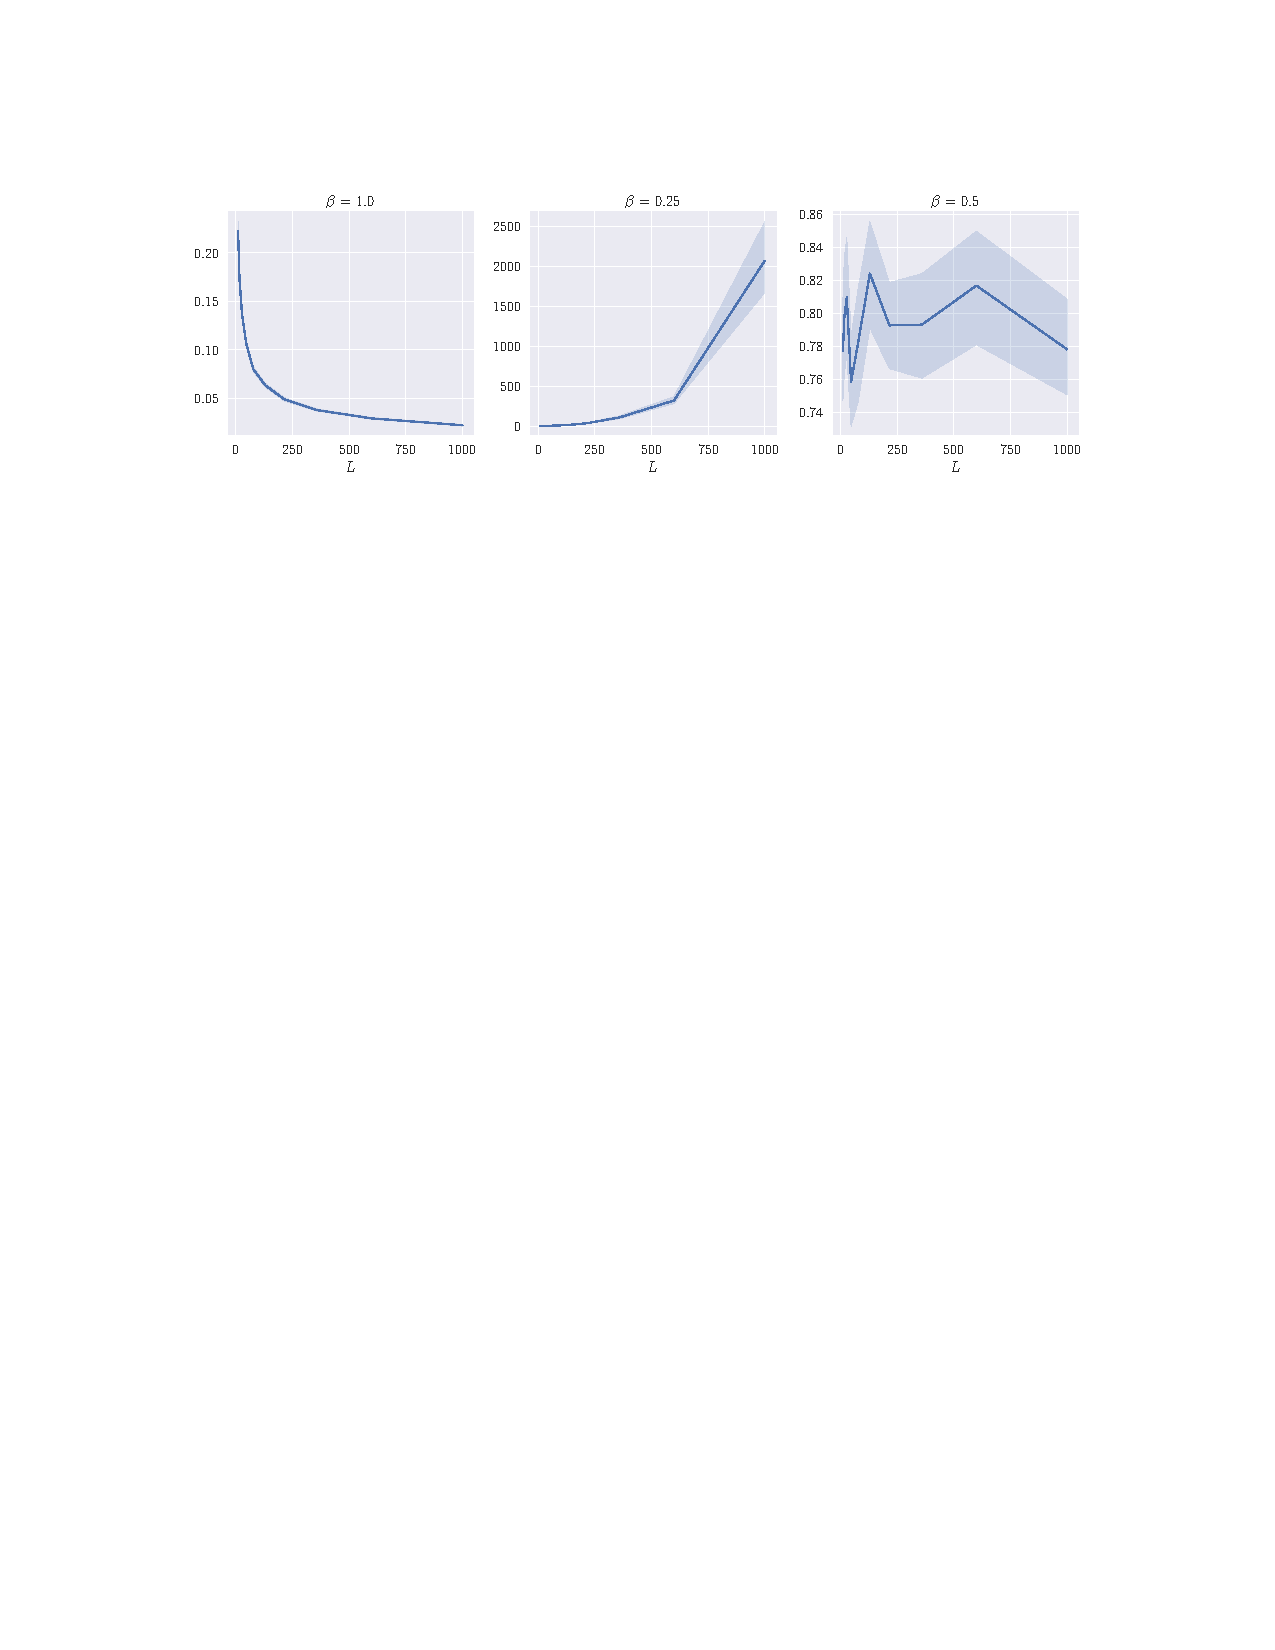
\includegraphics[width=.95\textwidth]{figs/figure_cor4.pdf}
    \caption{Illustration du corollaire \ref{cor4}. Évolution de $ \left\| h_L - h_0 \right\| / \left\| h_0 \right\| $ en fonction de $ L $ pour différente valeur de $ \beta  $.}
    \label{fig:cor4}
\end{figure}
\include{Partie2}
\chapter{Conclusion}
Ce tutoriel présente une analyse complète des défis liés à la mise à l'échelle dans les ResNets profonds. Il met en évidence l'importance du facteur de mise à l'échelle \(\alpha_L\), de l'analyse probabiliste et des informations fournies par les modèles en temps continu. En combinant une analyse théorique et des preuves empiriques, on parvient à une compréhension approfondie des mécanismes impliqués dans la formation des ResNets profonds. Cette approche ouvre la voie à la création d'architectures d'apprentissage profond plus efficaces et efficientes à l'avenir.

Premièrement, il convient de mentionner que les Resnets ont été un véritable exploit dans le domaine de l'apprentissage automatique complexe. Ils ont été les premiers modèles de réseaux neuronaux profonds à être entraînés avec succès avec un grand nombre de couches, ce qui a considérablement amélioré les performances. Étant donné son application étendue et son importance, il est essentiel de réfléchir à la manière de construire un cadre "parfait" afin d'éviter tout problème de disparition ou d'explosion de gradient lors de l'entraînement en profondeur, qui pourrait conduire à de mauvais résultats.

Deuxièmement, nous avons constaté, à travers de nombreuses expériences, que la répartition des valeurs initiales (les poids $(V_k)_{1\leqslant k \leqslant L }$ et $(\theta_k)_{1\leqslant k \leqslant L }$)joue un rôle crucial dans les résultats de l'entraînement. Par conséquent, il est impératif d'examiner attentivement la régularité de l'évolution des poids dans le processus de descente de gradient et son impact sur la dynamique de l'entraînement.

La relation entre le taux d'apprentissage et le facteur de mise à l'échelle $\alpha_{L}$ joue un rôle essentiel dans l'évaluation plus précise de la corrélation entre les performances du réseau formé et la mise à l'échelle.

\bibliographystyle{plain} % We choose the "plain" reference style
\bibliography{bib} % Entries are in the refs.bib file

\end{document}